\documentclass[UTF8]{ctexart}
\usepackage{amsmath,mathrsfs,amsfonts,mathtools}%引入数学宏
\usepackage{geometry}%引入编排宏
\usepackage{tikz}%引入画图宏
\usepackage{graphics}%引入排图宏
\usepackage{amssymb}%引入符号库
\usepackage{xtab,booktabs}%引入表格宏

\geometry{a4paper,centering,scale=.85}%A4纸,版心居中,长宽占比0.85


\begin{document}

\zihao{4}
\linespread{2}%行间距

\section{\heiti 函数与极限}

\subsection{\heiti 映射与函数}

本篇主要以了解为主,重点在函数的特性和附录部分.后面的双曲函数了解即可.

一、映射

1.映射的概念

定义1:设$X,Y$是两个非空集合,如果$\exists $一个法则$f$,使得$\forall x\in X$按法则$f$,在有唯一确定的元素$y\in Y$与之对应,那么称$f$为从$X$到$Y$的映射,记作$f:X\to Y$.

其中$y$称为元素$x$(在映射$f$)下的像,并记作$f(x)$,即$y=f(x)$;元素$x$称为元素$y$(在映射$f$下)的一个原像;

集合$X$称为映射$f$的定义域,记作$D_f$,即$D_f=X$;

$X$中所有元素的像组成的集合称为映射$f$的值域,记作$R_f$或$f(X)$,即$R_f=f(X)=\{ f(x)| x\in X\}$.

要注意的是

$(1)$映射三要素:定义域$D_f=X$,值域$R_f\displaystyle\subseteq Y$,对应法则$f$.三要素缺一不可

$(2)$元素$x$的像是唯一的,$y$的原像不一定是唯一的.

若$R_f=Y$,则映射$f$为满射;若$\forall x\in X$有一一对应的像$y\in R_f\subset  Y$,则称映射$f$为单射;若映射$f$即是满射又是单射则称映射$f$为一一映射$(\text{或满射})$

2、逆映射与复合映射

设$f$是$X$到$Y$的单射,由定义可得:对每$y\in R_f$,有唯一的$x\in X$,适合$f(x)=y$,于是定义一个从$R_f$到$X$的一个新映射即$g:R_f\to X$,对每个$y\in R_f$,规定$g(y)=x$,这个$x$满足$f(x)=y$.这个映射$g$称为$f$的逆映射,记作$f^{-1}$其定义域为$D_{f^{-1}}=R_f$,值域为$R_{f^{-1}}=X$

设有两个映射$g:X\to Y_1\ \ f:Y_2\to Z$,其中$Y_1\subseteq Y_2$,则由映射$g$和$f$可以定义一个从$X$到$Z$的一个对应法则,确定一个从$X$到$Z$的一个映射,这个映射称为由映射$g$和$f$构成的复合映射,记作$f\circ g$,即$f\circ g :X\to Z, \ \ \ (f\circ g)(x)=f\left[g(x)\right] ,\ x\in X$

由复合映射的定义可知:(1)满足条件$R_g\subseteq D_f$;(2)复合映射具有顺序性;(3)$f\circ g$有意义$g\circ f$不一定有意义,即使都有意义两映射也未必相同.

二、函数

1、函数的概念

定义2:设数集$D\subseteq  \mathbf{R} $,则称映射$f:D\to  \mathbf{R} $为定义在$D$上的函数,通常简记为$y=f(x),x\in D$,其中$x$称为自变量,$y$称为因变量,$D$称为定义域,记作$D_f=D$.

$y$称为函数$f$在$x$的函数值记作$f(x)$,因变量与自变量的关系称为函数关系,函数值全体组成的集合称为值域记作$R_f$或$f(D)$,即$R_f=f(D)=\left\{  y|y=f(x),x\in D \right\}$

不同的函数用不同的符号表示

定义域的确定:(1)由函数应用背景确定;(2)由函数的表达式确定(该定义域称为自然定义域)

函数的表示方法:(1)表格法(2)图形法(3)解析式法(又称公式法)

在自变量不同范围中,对应法则用不同的式子表示函数的函数叫分段函数

2、函数的性质

(1)、有界性

设函数$f(x)$的定义域为$D$,数集$X\subseteq D$:

如果$\exists K_{1}$,使$f(x)\leqslant K_{1}$对$\forall x\in X$都成立,那么称$f(x)$在$X$上有上界,而$K_{1}$是$f(x)$的一个上界;

如果$\exists K_{2}$,使$f(x)\geqslant  K_{1}$对$\forall x\in X$都成立,那么称$f(x)$在$X$上有下界,而$K_{2}$是$f(x)$的一个下界;

如果存在$M\in N_{+}$,使$|f(x)|\leqslant M$对$\forall x\in X$都成立那么称$f(x)$在$X$上有界,而$M$是$f(x)$的一个界,反之若$\nexists M\in N_{+}$就称称$f(x)$在$X$上无界.

注意:$f(x)$在$X$上有界.\ $\Longleftrightarrow $\ $f(x)$在$X$上有既有上界,又有下界.

(2)、单调性

设函数$f(x)$的定义域为$D$,区间$I\subseteq D$.如果$\forall $两点$x_{1},x_{2}\in I$:

当$x_{1}<x_{2}$时,恒有$f(x_{1})<f(x_{2})$那么称函数$f(x)$在$I$上单调增加的;

当$x_{1}<x_{2}$时,恒有$f(x_{1})>f(x_{2})$那么称函数$f(x)$在$I$上单调减少的;

在定义域内只单调增加或者只单调减少的函数称为单调函数.

(3)、函数的奇偶性

设函数$f(x)$的定义域$D$关于原点对称,对$\forall x\in D$:

若$f(-x)=f(x)$恒成立,那么称函数$f(x)$为偶函数,其图像关于$y$轴对称;

若$f(-x)=-f(x)$恒成立,那么称函数$f(x)$为奇函数,其图像关于原点对称;

(4)、周期性

设函数$f(x)$的定义域为$D$.如果$\exists l\in N_{+}$,使得对$\forall x\in D$有$(x+l)\in D$且$f(x+l)=f(x)$恒成立,那么称函数$f(x)$为周期函数,$l$称为函数$f(x)$的周期,通常我们说的周期是最小正周期.

要注意的是:并非所有函数都有最小正周期.

3、反函数与复合函数

反函数定义:设函数$f:D\to f(D)$是单射,则他存在逆映射$f^{-1}:f(D)\to D$,称此映射$f^{-1}$为函数$f$的反函数.

按定义,对每个$y\in f(D)$,有唯一的$x\in D$,使得$f(x)=y$,于是有$f^{-1}(x)$.也就是说反函数$f^{-1}$的对应法则是完全由函数$f$的对应法则所确定的.

一般的,$y=f(x)$,$x\in D$的反函数记成$y=f^{-1}(x),x\in D$.

若$f(x)$在定义域是单调函数,那么反函数$f^{-1}(x)$也是单调函数,且单调性相同

对反函数$y=f^{-1}(x)$来说,原函数$f(x)$称为直接函数.反函数与其直接函数关于直线$y=x$对称.

复合函数的定义:设函数$f(x)$的定义域为$D_{f}$,函数$u=g(x)$的定义域为$D_{g}$,且其值域$R_g\subseteq D_{f}$,则确定一个函数$y=f\left[g(x)\right]$,$x\in D$,称为由函数$u=g(x)$和函数$f(u)$构成的复合函数,它的定义域为$D_{g}$变量$u$称为中间变量.通常记为$f\circ g$,即$(f\circ g)(x)=f\left[g(x)\right]$.

注意的是:$f\left[f^{-1}(x)\right]=x$

4、函数的运算

设函数$f(x),g(x)$的定义域依次为$D_{f},D_{g},D=D_{f}\cap D_{g}=\varnothing $,我们可定义两个函数计算

和$($差$)$运算$f\pm g$:\ \ \ \ \ \ \ $(f\pm g)(x)=f(x)\pm g(x),x\in D$;

积$f\cdot g$:\ \ \ \ \ \ \ \ \ \ \ \ \ \ \ \ \ \ \ \ $(f\cdot g)(x)=f(x)\cdot g(x),x\in D$;\\

商$\displaystyle \frac{f}{g}$:\ \ \ \ \ \ \ \ \ \ \ \ \ \ \ \ \ \ \ \ \ \ \ $\displaystyle (\frac{f}{g})(x)=\frac{f(x)}{g(x)},x\in D\setminus \left\{x|g(x)=0,x\in D\right\} $\\

5、初等函数

基本初等函数

常数函数:$y=C(C\text{是常数})$;

幂函数:$y=x^{\mu }(\mu \in \mathbf{R} \text{是常数})$;

指数函数:$y=a^{x}(a>0\text{且}a\neq 1)$;

对数函数$y=\log _{a}x(a>0\text{且}a\neq 1,\text{当}a=e\text{时,记为}\ln x,\text{当}a=10\text{时,记为}\lg x)$;

三角函数:如$y=\sin x,y=\cos x,y=\tan x$等;

反三角函数:如$y=\arccos x,y=\arcsin x,y=\arctan x$等;

由基本初等函数经过有限次的四则运算和有限次的复合构成的式子称为初等函数.\\

{\heiti 附录}

该附录对基本初等函数、不等式进行知识补充,以及本节出现的函数图像

1、不等式(主要是不等式链和其他重要不等式,一般用于无穷级数或者求部分函数的有界性)

不等式链:\\

$\displaystyle  \sqrt{\frac{x_{1}^{2}+x_{2}^{2}+\ldots +x_{n}^{2}}{n}}\geqslant  \frac{x_{1}+x_{2}+\ldots +x_{n}}{n}\geqslant \sqrt[n]{x_{1}x_{2}\ldots x_{n} } \geqslant \frac{n}{\frac{1}{x_{1}}+\frac{1}{x_{2}}+\ldots \frac{1}{x_{n}}} $

当且仅当$x_{1}=x_{2}=\ldots =x_{n}$时等式成立\\

柯西不等式

$\displaystyle (x_{1}^{2}+x_{2}^{2}+\ldots +x_{n}^{2})(y_{1}^{2}+y_{2}^{2}+\ldots +y_{n}^{2})\geqslant (x_{1}y_{1}+x_{2}y_{2}+\ldots x_{n}y_{n})$

当且仅当$x_{i}(i=1,2,\ldots ,n)=0$或$y_{i}(i=1,2,\ldots ,n)=0$时或$x_{i}=\lambda y_{i}(i=1,2,\ldots ,n)$时等式成立$(\text{两元形式:当}x_{1}y_{2}=x_{2}y_{1}\text{时等号成立})$

2、基本初等函数(不对高中见过的函数的定义域和值域说明,三角函数、指数函数、对数函数单独说明)

常数函数:$y=C(C\text{是常数})$;

幂函数:$y=x^{\mu }(\mu \in \mathbf{R} \text{是常数})$;



\begin{figure}[htb]
    \centering
    \begin{tikzpicture}
        \begin{scope}
            \draw [->](-2,0)--(2,0);
            \draw [->](0,-2)--(0,2);
            \node at (-.25,-.25){$O$};
            \draw (-2,1)--(2,1);
            \node at (-2.75,1.25){$y=C$};
            \node at (-.25,.75){$C$};
        \end{scope}
        
        \begin{scope}[xshift=8cm]
            \draw [->](-2,0)--(2,0);
            \draw [->](0,-2)--(0,2);
            \node at (.25,.25){$O$};
            \draw[domain=0:2, samples=1000, thick,color=black]
              plot(\x,{\x^0.5});
            \node[color=black] at (3.3,1.55){$\displaystyle y=\sqrt{x}=x^{\frac{1}{2}} $};
            \draw[domain=0.575:2, samples=1000, thick,color=magenta]
              plot(\x,{\x^-1});
            \draw[domain=-2.:-0.575, samples=1000, thick,color=magenta]
              plot(\x,{\x^-1});
            \node[color=magenta] at (-3,-.3){$\displaystyle y=\frac{1}{x}=x^{-1}$};
            \draw[domain=-2:2, samples=1000, thick,color=cyan]
              plot(\x,{\x});  
            \node[color=cyan] at (2.5,1.85){$y=x$} ; 
            \draw[domain=-1.414:1.414, samples=1000, thick,color=green]
              plot(\x,{\x*\x});  
            \node[color=green] at (2,2.3){$y=x^2$} ;
            \draw[domain=-1.26:1.26, samples=1000, thick,color=red]
              plot(\x,{\x*\x*\x});  
            \node [color=red] at (-1.5,-2.3){$y=x^3$} ;
            
            
        \end{scope}    
        \end{tikzpicture}
    \caption{常数函数(左),部分常见的幂函数(右)}
    \label{<label>}
\end{figure}

3、指数与指数函数

指数法则

若$a>0,b>0,n\text{、}m\text{是常数}$那么$\displaystyle a^{n}\cdot a^{m}=a^{n+m},\frac{a^{n}}{a^{m}}=a^{n-m},(a^{n})^{m}=a^{nm},$\\$\displaystyle a^{n}\cdot b^{n}=(ab)^{n},\frac{a^{n}}{b^{n}}=(\frac{a}{b})^{n},a^1=a,a^0=1$\\

指数换底公式(洛必达法则会用上,题外话:对数的运算法则就是利用这个推出来的)

对$a>0,b>0,x>0$有$\displaystyle a^x=b^{\log_{b}x}$

指数函数:$y=a^{x}(a>0\text{且}a\neq 1),D_{f}=\mathbf{R} ,R_{f}=(0,+\infty )$;

当$a$离$1$越远,图像越陡峭,图像横过点$(0,1)$.

4、对数与对数函数

对数法则

若$a>0,a\neq 1,b>0,b\neq 1,x>0,y>0,n>0,m>0$那么

$\displaystyle \log _{a}(xy)=\log _{a}(x)+\log _{a}(y),\log _{a}(\frac{x}{y})=\log _{a}(x)-\log _{a}(y),\log _{a^n}(x^m)=\frac{m}{n}\log _{a}(x),$

对数换底公式$\displaystyle \log _{a}(x)=\frac{\log _{b}(x)}{\log _{b}(a)}$

对数函数$y=\log _{a}x(a>0\text{且}a\neq 1,),D_{f}=(0,+\infty ) ,R_{f}=\mathbf{R} $

$\text{当}a=e\text{时,记为}\ln x(\text{自然对数}),\text{当}a=10\text{时,记为}\lg x(\text{常用对数})$;

$a$离$1$越近,图像越陡峭,图像横过点$(1,0)$.

指数和对数的转换$y=a^{x}\Leftrightarrow x=\log _{a}(y)(a>0,a\neq 1)$

\begin{figure}[htb]
    \centering
    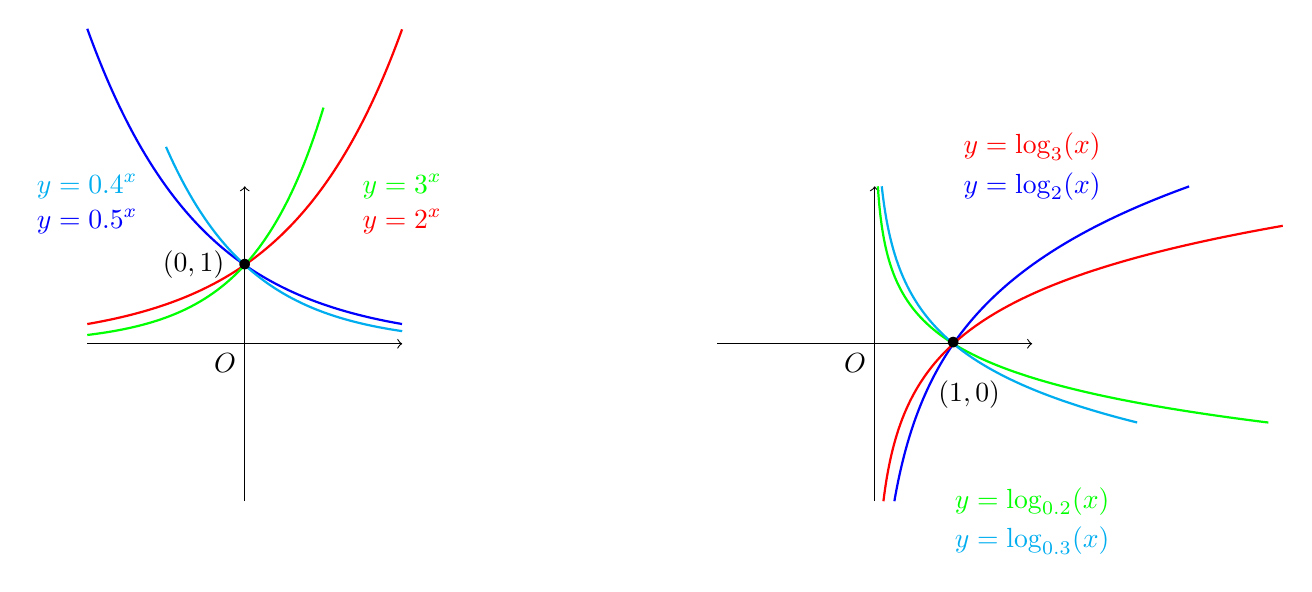
\begin{tikzpicture}
        \begin{scope}
            \draw [->](-2,0)--(2,0);
            \draw [->](0,-2)--(0,2);
            \node at (-.25,-.25){$O$};
            \draw[domain=-2:2, samples=1000, thick,color=red]
              plot(\x,{2^\x});
            \node[color=red] at (2,1.55){$\displaystyle y=2^{x} $};
            \draw[domain=-2:1, samples=1000, thick,color=green]
              plot(\x,{3^\x});
            \node[color=green] at (2,2){$\displaystyle y=3^{x} $};
            \draw[domain=-2:2, samples=1000, thick,color=blue]
              plot(\x,{0.5^\x});
            \node[color=blue] at (-2,1.55){$\displaystyle y=0.5^{x} $};
            \draw[domain=-1:2, samples=1000, thick,draw=cyan]
              plot(\x,{0.4^\x});
            \node[color=cyan] at (-2,2){$\displaystyle y=0.4^{x} $};
            \node at (0,1){$\bullet $};
            \node at (-.65,1){$(0,1)$};
        \end{scope} 
        \begin{scope}[xshift=8cm]
            \draw [->](-2,0)--(2,0);
            \draw [->](0,-2)--(0,2);
            \node at (-.25,-.25){$O$};
            \draw[domain=-2:2, samples=1000, thick,color=blue]
              plot({2^\x},\x);
            \node[color=blue] at (2,2){$\displaystyle y=\log _{2}(x) $};
            \draw[domain=-2:1.5, samples=1000, thick,color=red]
              plot({3^\x},\x);
            \node[color=red] at (2,2.5){$\displaystyle y=\log _{3}(x) $};
            \draw[domain=-1:2, samples=1000, thick,color=green]
              plot({0.2^\x},\x);
            \node[color=green] at (2,-2){$\displaystyle y=\log _{0.2}(x) $};
            \draw[domain=-1:2, samples=1000, thick,color=cyan]
              plot({0.3^\x},\x);
            \node[color=cyan] at (2,-2.5){$\displaystyle y=\log _{0.3}(x) $};
            \node at (1,0){$\bullet $};
            \node at (1.2,-.65){$(1,0)$};
        \end{scope}
    \end{tikzpicture}
    \caption{指数函数(左)对数函数(右)}
    \label{<label>}
\end{figure}

5、三角函数和反三角函数(重点和难点,微积分常用三角函数及其公式进行解题尤其是积分,我们统一用弧度制表达)

三角函数

正弦,余弦,正切:$\displaystyle y=\sin x ,y=\cos x ,y\tan x=\frac{\sin x}{\cos x} $

正割,余割,余切$\displaystyle y=\sec x=\frac{1}{\cos x} ,y=\text{cse} x =\frac{1}{\sin x},y=\cot x=\frac{1}{\tan x}$\\

正弦、余弦的定义域为$\mathbf{R} $,正切、正割割的定义域是$x\neq \pm \frac{(2n-1)\pi}{2}(n=1,2\ldots )$,\\余割、余切的定义域是$x\neq \pm 2n\pi(n=0,1,2\ldots)$

正弦、余弦的值域为$\left[1,1\right] $,正切、余切的值域为$\mathbf{R} $,\\正割、余割的值域为$ \left(-\infty ,1 \right]\cup\left[1,+\infty \right)  $

正弦、余弦、正割、余割的周期为$2\pi$,正切、余切的周期为$\pi$

$T=\frac{2\pi}{\omega }$

在坐标系中$(x,y)\Leftrightarrow (r\cos \theta ,r\sin \theta )$

其中$x^2+y^2=r^2,\theta \text{是点与原点形成的直线与$x$轴形成的夹角}$

三角公式(数量非常多,但是大多数都是由公式推导出来只要记住4、5个我叫背公式就行,剩下的自己推导多了就能记住了,):

公式1:$ \sin^2 x+\cos^2 x=1$(背)\ \ \ $1+\cot^2 x=\text{csc}^2 x$\ \ \ $\tan^2 x +1=\sec^2 x$

公式2:$\cos(A\pm B)=\cos A \cos B \mp \sin A \sin B$(背(A+B)的就行),

\ \ \ \ \ \ \ \ \ $\sin (A\pm B)=\sin A \cos B \pm\cos A \sin B$(背(A+B)的就行),\\

\ \ \ \ \ \ \ \ \ $\displaystyle \tan (A\pm B)=\frac{\tan A \pm \tan B}{1\mp \tan A\tan B}$\\

公式3(半角公式,变次公式)(正负号由$\theta $决定):$\displaystyle \cos ^{2}\theta =\frac{1+\cos 2\theta }{2},\sin ^{2}\theta =\frac{1-\cos 2\theta }{2}$\\

\ \ \ \ \ \ \ \ \ \ \ \ \ \ \ \ \ \ \ \ \ \ \ $\displaystyle \tan ^{2}\theta =(\frac{\sin \theta}{1+\cos \theta})^{2}=(\frac{1-\cos \theta}{\sin \theta})^{2}=\frac{1-\cos \theta}{1+\cos \theta}$\\

公式4(倍角公式):$\displaystyle \sin 2\theta =2\sin\theta \cos \theta =\frac{2\tan \theta}{1+\tan^{2}\theta}$\\

\ \ \ \ \ \ \ \ \ \ \ \ \ \ \ \ \ \ \ \ \ \ \ $\displaystyle \cos 2\theta =\cos ^{2}\theta -\sin ^{2}\theta =2\cos ^{2}\theta -1=1-2\sin^{2}\theta=\frac{1-\tan^{2}\theta}{1+\tan^{2}\theta}$\\

\ \ \ \ \ \ \ \ \ \ \ \ \ \ \ \ \ \ \ \ \ \ \ $\displaystyle \tan 2\theta=\frac{2\tan \theta}{1-\tan^{2}\theta}$\\

公式4(和差化积):$\displaystyle \sin A\pm \sin B=2\sin(\frac{A\pm B}{2})\cos(\frac{A\mp B}{2})$\\

\ \ \ \ \ \ \ \ \ \ \ \ \ \ \ \ \ \ \ \ \ \ \ $\displaystyle \cos A+\cos B=2\cos(\frac{A+B}{2})\cos(\frac{A-B}{2})$\\

\ \ \ \ \ \ \ \ \ \ \ \ \ \ \ \ \ \ \ \ \ \ \ $\displaystyle \cos A-\cos B=-2\sin(\frac{A+B}{2})\sin(\frac{A-B}{2})$\\

公式4(积化和差)$\displaystyle \sin A\cos B=\frac{1}{2}\left[\sin(A+B)+\sin(A-B)\right] $\\

\ \ \ \ \ \ \ \ \ \ \ \ \ \ \ \ \ \ \ \ \ \ \ $\displaystyle \cos A\cos B=\frac{1}{2}\left[\cos(A+B)+\cos(A-B)\right] $\\

\ \ \ \ \ \ \ \ \ \ \ \ \ \ \ \ \ \ \ \ \ \ \ $\displaystyle \sin A\sin B=\frac{1}{2}\left[\cos(A+B)-\cos(A-B)\right] $\\

\begin{figure}[htb]
  \centering
  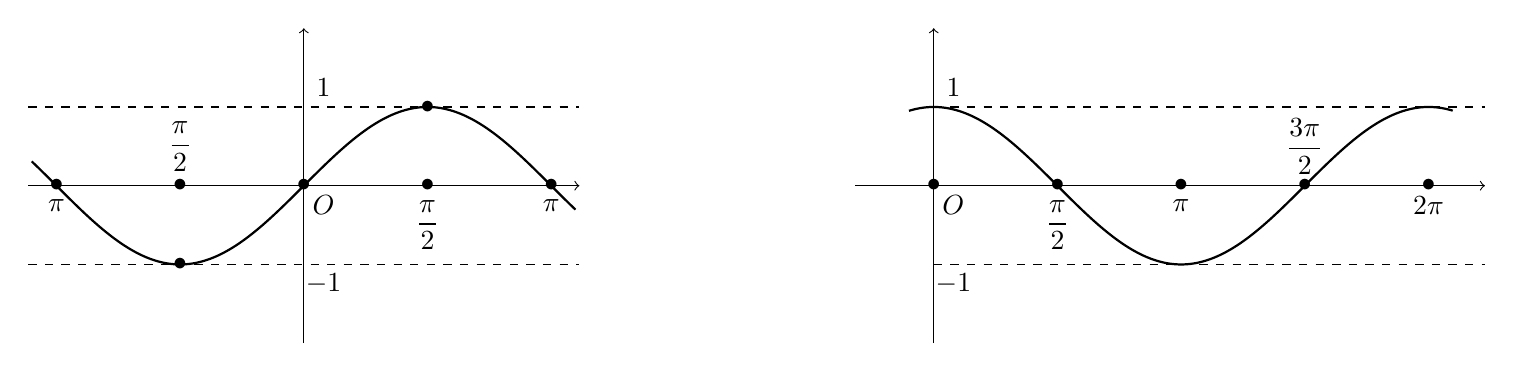
\begin{tikzpicture}
      \begin{scope}
          \draw [->](-3.5,0)--(3.5,0);
          \draw [->](0,-2)--(0,2);
          \draw [dashed](-3.5,1)--(3.5,1);
          \draw [dashed](-3.5,-1)--(3.5,-1);
          \node at (.25,-.25){$O$};
          \draw[domain=-pi-pi/10:pi+pi/10, samples=1000, thick]
              plot(\x,{sin (\x r)});
          \node at (0,0){$\bullet $};
          \node at (pi,0){$\bullet $};
          \node at (pi,-.25){$\pi $};
          \node at (pi/2,0){$\bullet $};
          \node at (pi/2,1){$\bullet $};
          \node at (pi/2,-.5){$ \displaystyle\frac{\pi}{2}$};
          \node at (-pi,0){$\bullet $};
          \node at (-pi,-.25){$\pi $};
          \node at (-pi/2,0){$\bullet $};
          \node at (-pi/2,.5){$\displaystyle\frac{\pi}{2} $};
          \node at (-pi/2,-1){$\bullet $};
          \node at (.25,1.25){$1 $};
          \node at (.25,-1.25){$-1 $};
      \end{scope} 
      \begin{scope}[xshift=8cm]
        \draw [->](-1,0)--(7,0);
        \draw [->](0,-2)--(0,2);
        \draw [dashed](0,1)--(7,1);
        \draw [dashed](0,-1)--(7,-1);
        \node at (.25,-.25){$O$};
        \draw[domain=-pi/10:pi+pi+pi/10, samples=1000, thick]
            plot(\x,{cos (\x r)});
        \node at (0,0){$\bullet $};
        \node at (pi,0){$\bullet $};
        \node at (pi,-.25){$\pi $};
        \node at (pi/2,0){$\bullet $};
        \node at (pi/2,-.5){$ \displaystyle\frac{\pi}{2}$};
        \node at (pi+pi,0){$\bullet $};
        \node at (pi+pi,-.25){$2\pi $};
        \node at (pi/2+pi,0){$\bullet $};
        \node at (pi/2+pi,.5){$\displaystyle\frac{3\pi}{2} $};
        \node at (.25,1.25){$1 $};
        \node at (.25,-1.25){$-1 $};
      \end{scope}
  \end{tikzpicture}
  \caption{正弦函数(左)、余弦函数(右)图像(部分)}
  \label{<label>}
\end{figure}

\begin{figure}[htb]
  \centering
  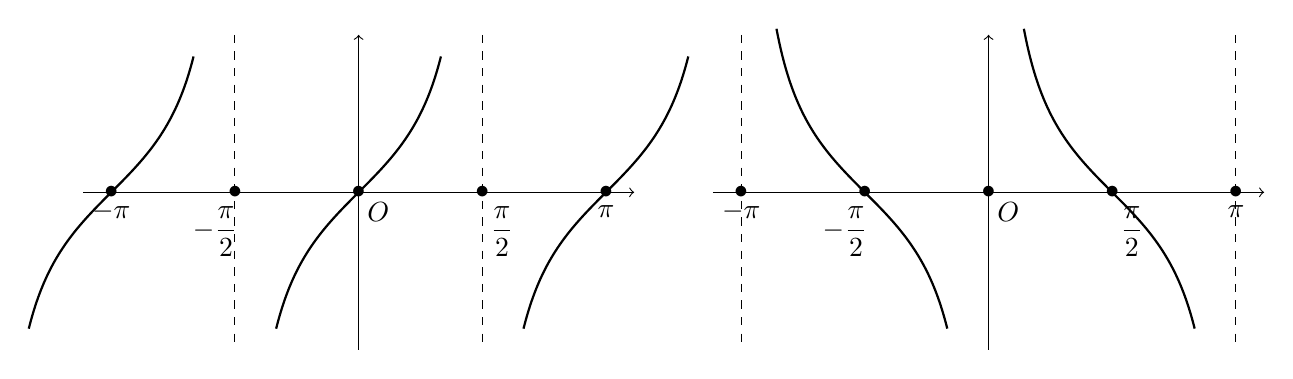
\begin{tikzpicture}
      \begin{scope}
          \draw [->](-3.5,0)--(3.5,0);
          \draw [->](0,-2)--(0,2);
          \draw [dashed](pi/2,2)--(pi/2,-2);
          \draw [dashed](-pi/2,2)--(-pi/2,-2);
          \node at (.25,-.25){$O$};
          \draw[domain=-pi/3:pi/3, samples=1000, thick]
              plot(\x,{tan (\x r)});
          \draw[domain=pi/3+pi/3:pi/3+pi, samples=1000, thick]
              plot(\x,{tan (\x r)});
          \draw[domain=-pi/3-pi:pi/3-pi, samples=1000, thick]
              plot(\x,{tan (\x r)}); 
          \node at (0,0){$\bullet $};
          \node at (pi,0){$\bullet $};
          \node at (pi,-.25){$\pi $};
          \node at (pi/2,0){$\bullet $};
          \node at (pi/2+.25,-.5){$ \displaystyle\frac{\pi}{2}$};
          \node at (-pi,0){$\bullet $};
          \node at (-pi,-.25){$-\pi $};
          \node at (-pi/2,0){$\bullet $};
          \node at (-pi/2-.25,-.5){$\displaystyle -\frac{\pi}{2} $};  
      \end{scope} 
      \begin{scope}[xshift=8cm]
        \draw [->](-3.5,0)--(3.5,0);
        \draw [->](0,-2)--(0,2);
        \node at (.25,-.25){$O$};
        \draw [dashed](pi,2)--(pi,-2);
        \draw [dashed](-pi,2)--(-pi,-2);
        \draw[domain=pi/7:pi/2+pi/3, samples=1000, thick]
            plot(\x,{cot(\x r) });
        \draw[domain=pi/7-pi:pi/2+pi/3-pi, samples=1000, thick]
            plot(\x,{cot(\x r) });
        \node at (0,0){$\bullet $};
        \node at (pi,0){$\bullet $};
        \node at (pi,-.25){$\pi $};
        \node at (pi/2,0){$\bullet $};
        \node at (pi/2+.25,-.5){$ \displaystyle\frac{\pi}{2}$};
        \node at (-pi,0){$\bullet $};
        \node at (-pi,-.25){$-\pi $};
        \node at (-pi/2,0){$\bullet $};
        \node at (-pi/2-.25,-.5){$\displaystyle -\frac{\pi}{2} $};   
      \end{scope}
  \end{tikzpicture}
  \caption{正切函数(左)、余切函数(右)图像(部分)}
  \label{<label>}
\end{figure}


\begin{figure}[htb]
  \centering
  \begin{tikzpicture}
      \begin{scope}
          \draw [->](-3.5,0)--(3.5,0);
          \draw [->](0,-2)--(0,2);
          \draw [dashed](pi/2,2)--(pi/2,-2);
          \draw [dashed](-pi/2,2)--(-pi/2,-2);
          \node at (.25,-.25){$O$};
          \draw [dashed](-3.5,1)--(3.5,1);
          \draw [dashed](-3.5,-1)--(3.5,-1);
          \node at (.25,1.25){$1 $};
          \node at (.25,-1.25){$-1 $};
          \draw[domain=-pi/3:pi/3, samples=1000, thick]
              plot(\x,{sec (\x r)});
          \draw[domain=-pi/3+pi:pi, samples=1000, thick]
              plot(\x,{sec (\x r)});
          \draw[domain=-pi:pi/3-pi, samples=1000, thick]
              plot(\x,{sec (\x r)});         
          \node at (0,0){$\bullet $};
          \node at (pi,0){$\bullet $};
          \node at (pi,-.25){$\pi $};
          \node at (pi/2,0){$\bullet $};
          \node at (pi/2+.25,-.5){$ \displaystyle\frac{\pi}{2}$};
          \node at (-pi,0){$\bullet $};
          \node at (-pi,-.25){$-\pi $};
          \node at (-pi/2,0){$\bullet $};
          \node at (-pi/2-.25,-.5){$\displaystyle -\frac{\pi}{2} $};  
      \end{scope} 
      \begin{scope}[xshift=8cm]
        \draw [->](-3.5,0)--(3.5,0);
        \draw [->](0,-2)--(0,2);
        \node at (.25,-.25){$O$};
        \draw [dashed](pi,2)--(pi,-2);
        \draw [dashed](-pi,2)--(-pi,-2);
        \draw [dashed](-3.5,1)--(3.5,1);
        \draw [dashed](-3.5,-1)--(3.5,-1);
        \node at (.25,1.25){$1 $};
        \node at (.25,-1.25){$-1 $};
        \draw[domain=pi/8:pi/2+pi/3+pi/100, samples=1000, thick]
            plot(\x,{sin(\x r)^-1 });
        \draw[domain=pi/8-pi:-pi/2+pi/3+pi/100, samples=1000, thick]
            plot(\x,{sin(\x r)^-1 });            
        \node at (0,0){$\bullet $};
        \node at (pi,0){$\bullet $};
        \node at (pi,-.25){$\pi $};
        \node at (pi/2,0){$\bullet $};
        \node at (pi/2+.25,-.5){$ \displaystyle\frac{\pi}{2}$};
        \node at (-pi,0){$\bullet $};
        \node at (-pi,-.25){$-\pi $};
        \node at (-pi/2,0){$\bullet $};
        \node at (-pi/2-.25,-.5){$\displaystyle -\frac{\pi}{2} $};   
      \end{scope}
  \end{tikzpicture}
  \caption{正切函数(左)、余切函数(右)图像(部分)}
  \label{<label>}
\end{figure}

\newpage

反三角函数

将三角函数的定义域进行限制,我们就可以定义出三角函数的反函数,我们称之为反三角函数.

正弦函数$\displaystyle y=\sin x ,x\in \left[-\frac{\pi}{2},\frac{\pi}{2}\right] \Longrightarrow $反正弦函数$\displaystyle y=\arcsin x,x\in \left[-1,1\right] ,\\y\in\left[-\frac{\pi}{2},\frac{\pi}{2}\right] $\\

余弦函数$\displaystyle y=\cos x ,x\in \left[0,\pi\right] \Longrightarrow $反余弦函数$\displaystyle y=\arccos x,x\in \left[-1,1\right] ,y\in\left[0,\pi\right] $\\

正切函数$\displaystyle y=\tan x ,x\in (-\frac{\pi}{2},\frac{\pi}{2}) \Longrightarrow $反正切函数$\displaystyle y=\arctan x,x\in \mathbf{R}  ,\\y\in (-\frac{\pi}{2},\frac{\pi}{2}) $\\

余切函数$\displaystyle y=\cot x ,x\in (-\frac{\pi}{2},\frac{\pi}{2}) \Longrightarrow $反余切函数$\displaystyle y=\text{arccot} x,x\in \mathbf{R}  ,y\in (0,\pi ) $\\

\begin{figure}[htb]
  \centering
  \begin{tikzpicture}
      \begin{scope}
          \draw [->](-2,0)--(2,0);
          \draw [->](0,-2)--(0,2);
          \draw [dashed](-2,pi/2)--(2,pi/2);
          \draw [dashed](-2,-pi/2)--(2,-pi/2);
         
          \node at (.25,-.25){$O$};
          \node at (0,pi/2){$\bullet $};
          \node at (0,-pi/2){$\bullet $};
          \node at (.25,pi/2){$\displaystyle\frac{\pi}{2}$};
          \node at (.25,-pi/2){$\displaystyle -\frac{\pi}{2} $};
          \node at (1,-.25){$1$} ;
          \node at (1,0){$\bullet $};
          \node at (-1,-.25){$-1$} ;
          \node at (-1,0){$\bullet $};
          \draw[domain=-pi/2:pi/2, samples=1000, thick]
              plot({sin (\x r)},\x);
           
      \end{scope} 
      \begin{scope}[xshift=8cm,yshift=-1.48cm]
        \draw [->](-2,0)--(2,0);
        \draw [->](0,-1)--(0,3.5);
        \node at (.25,-.25){$O$};
        \draw [dashed](2,pi)--(-2,pi);
        \node at (0,pi){$\bullet $};
        \node at (.25,pi+.2){$\pi$};
        \node at (.25,pi/2+.2){$\displaystyle\frac{\pi}{2}$};
        \node at (0,pi/2){$\bullet $}; 
        \node at (1,-.25){$1$} ;
        \node at (1,0){$\bullet $};  
        \draw[domain=0:pi, samples=1000, thick]
            plot({cos(\x r) },\x);
                    
        
      \end{scope}
  \end{tikzpicture}
  \caption{反正弦函数函数(左)、反余弦函数(右)图像(部分)}
  \label{<label>}
\end{figure}

\begin{figure}[htb]
  \centering
  \begin{tikzpicture}
      \begin{scope}
          \draw [->](-2,0)--(2,0);
          \draw [->](0,-2)--(0,2);
          \draw [dashed](-2,pi/2)--(2,pi/2);
          \draw [dashed](-2,-pi/2)--(2,-pi/2);
         
          \node at (.25,-.25){$O$};
          \node at (0,pi/2){$\bullet $};
          \node at (0,-pi/2){$\bullet $};
          \node at (.25,pi/2){$\displaystyle\frac{\pi}{2}$};
          \node at (.25,-pi/2){$\displaystyle -\frac{\pi}{2} $};
          \node at (1,-.25){$1$} ;
          \node at (1,0){$\bullet $};
          \node at (-1,-.25){$-1$} ;
          \node at (-1,0){$\bullet $};
          \draw[domain=-pi/3:pi/3, samples=1000, thick]
              plot({tan (\x r)},\x);
           
      \end{scope} 
      \begin{scope}[xshift=8cm,yshift=-1.48cm]
        \draw [->](-2,0)--(2,0);
        \draw [->](0,-1)--(0,3.5);
        \node at (.25,-.25){$O$};
        \draw [dashed](2,pi)--(-2,pi);
        \node at (0,pi){$\bullet $};
        \node at (.25,pi+.2){$\pi$};
        \node at (.25,pi/2+.2){$\displaystyle\frac{\pi}{2}$};
        \node at (0,pi/2){$\bullet $}; 
        \node at (1,-.25){$1$} ;
        \node at (1,0){$\bullet $};  
        \draw[domain=pi/10:pi-pi/10, samples=1000, thick]
            plot({cot(\x r) },\x);
                    
        
      \end{scope}
  \end{tikzpicture}
  \caption{反正切函数函数(左)、反余切函数(右)图像(部分)}
  \label{<label>}
\end{figure}

\newpage

其他函数(主要是绝对值函数,)

a.绝对值函数
$f(x)=\left\lvert x\right\rvert =\begin{dcases}
x,&x>0;\\-x,&x<0.    
\end{dcases}$%列式子
范围
$\begin{dcases}
D=R\\R_f=\left[0,\infty \right)%半开半闭区间
\end{dcases}$%表示定义域和值域

同时绝对值还表示两点的距离(重点)

\begin{figure}[htbp]%绝对值函数图像,文章中
    \centering
\begin{tikzpicture}[>=latex]
  \begin{scope}
   \draw[->](-3,0)--(3,0)node[right]{$x$};%画x轴
\draw[->](0,-1)--(0,3)node[right]{$y$};%画y轴
\draw(0,0)--(2,2);
\draw(0,0)--(-2,2)node[left]{$\vert x\vert $};
\draw(-.2,-.2)node{$O$};%表明原点

   \end{scope}             
   \begin{scope}[xshift=8cm]
   \draw[->](-2,0)--(2,0)node[right]{$x$};
   \draw[->](0,-2)--(0,2)node[right]{$y$};
   \draw(0,1)node[left]{$1$}--(2,1);
   \draw(0,1)node{$\circ $};
  \draw(0,-1)node[right]{$-1$}--(-2,-1);
  \draw(0,-1)node{$\circ $};
  \draw(-0.2,-0.2)node{$O$};
  \draw(0,0)node{$\bullet $};
                
    
  \end{scope}
  
\end{tikzpicture}
\caption{绝对值函数(左)、符号函数函数(右)图像(部分)}
\end{figure}

b.符号函数
$f(x)=sgn x=\begin{dcases}
    -1,&x<0;\\0,&x=0;\\1,&x>0.
\end{dcases}$
范围
$\begin{dcases}
D=R\\R_f=\{-1,0,1\}
\end{dcases}$

注意:$sgnx\cdot |x| =x$\\

c.取整函数

我们将不超过$x$的最大整数称为$x$的整数部分称为$x$的整数,可定义函数$f(x)=[x]$,该函数称为取整函数,其图像称为阶梯曲线.

$f(x)=[x]$
\begin{figure}[htbp]
    \centering
\begin{tikzpicture}
\draw[->](-2,0)--(3,0)node[right]{$x$};
\draw[->](0,-2)--(0,3)node[right]{$y$};
\foreach \x in{-1,1,2}
{
    \draw (0,\x)node[left]{$\x$}--(.1,\x);
    \draw (\x,0)node[below]{$\x$}--(\x,.1);
}%画刻度
\draw(1,1)node{$\bullet $}--(2,1)node{$\circ $};
\draw(0,0)node{$\bullet $}--(1,0)node{$\circ $};
\draw(-1,-1)node{$\bullet $}--(0,-1)node{$\circ $};
\draw(-0.2,-0.2)node{$O$};
\end{tikzpicture}
    \caption{取整函数}
\end{figure}\\

狄利克雷函数$D(x) = \begin{dcases}
  1,&x \in Q;\\0,&x \in Q^c.    
  \end{dcases}$
$Q^c$是无理数

$\forall r \in R$是其周期,所以该函数无最小正周期.

邻域(了解就好,因为后面会涉及到所以就讲一下)

以$x_{0}$为中心的$\forall $开区间称为点$x_{0}$的邻域,记作$\bigcup (x_{0})$,在$\bigcup (x_{0})$中去掉中心$x_{0}$后,称为点$x_{0}$的去心邻域,记作$\bigcup \limits^{\circ }(x_{0})$

设$x_{0}\in \mathbf{R} ,\delta >0$,开区间$(x_{0}-\delta ,x_{0}+\delta ) $称为点$x_{0}$的$\delta $邻域,记作$\bigcup (x_{0},\delta )$,在$\bigcup (x_{0},\delta )$中去掉中心$x_{0}$后,称为点$x_{0}$的去心$\delta $邻域,记作$\bigcup \limits^{\circ }(x_{0},\delta )$






















































\end{document}